%### Einstellungen ###################################
\documentclass[a4paper,12pt,oneside]{scrreprt}

%### Packages und Configuration ######################
\usepackage[left= 3cm, right = 2cm, bottom = 2cm, top = 2cm]{geometry}
%für das Umschmiegen des Textes um ein Bild
\usepackage{wrapfig}
\usepackage[utf8]{inputenc}
\usepackage{xcolor}
\usepackage[ngerman]{babel}

\usepackage[chapter]{minted}
\usemintedstyle{solarized-light}
\setminted{linenos=true}

\usepackage[T1]{fontenc}
\usepackage{graphicx, subfig}
\graphicspath{{img/}}

\usepackage{fancyhdr}
\usepackage{lmodern}
\renewcommand*\familydefault{\sfdefault}

\usepackage{color}
\usepackage{underscore}
\usepackage{acronym}
% zusätzliche Schriftzeichen der American Mathematical Society
\usepackage{amsfonts}
\usepackage{amsmath}


%### Code Listing Style ##############################
\usepackage{listings}
\definecolor{backcolour}{rgb}{0.95,0.95,0.92}              
\definecolor{commentcolor}{rgb}{0.497495, 0.497587, 0.497464}
\definecolor{keywordcolor}{rgb}{0.000000, 0.000000, 0.635294}
\definecolor{ndkeywordcolor}{rgb}{0,0.6,0.2}
\definecolor{numbercolor}{rgb}{0.5,0.5,0.5}
\definecolor{stringcolor}{rgb}{0.6,0.3,0.1}

\definecolor{deepred}{rgb}{0.6,0,0}
\definecolor{purple}{rgb}{0.58,0,0.82}

% Einstellen der Benutzerdefinierten Code-Farben
\lstdefinestyle{mystyle}{
    backgroundcolor=\color{backcolour},   
    commentstyle=\color{commentcolor},
    otherkeywords={self},
    keywordstyle=\color{keywordcolor}\bfseries,
  	ndkeywordstyle=\color{ndkeywordcolor}\bfseries,
    numberstyle=\tiny\color{numbercolor},
    stringstyle=\color{stringcolor}\bfseries,
    emph={import},
    emphstyle=\color{deepred},
    basicstyle=\footnotesize,  
    frame=single,
    breakatwhitespace=false,         
    breaklines=false,                 
    captionpos=b,                    
    keepspaces=true,                 
    numbers=left,                    
    numbersep=5pt,                                        
    showspaces=false,                
    showstringspaces=false,
    showtabs=false,                  
    tabsize=2,
   postbreak=\mbox{\textcolor{deepred}{$\hookrightarrow$}\space}
}
\lstset{style=mystyle}
\renewcommand{\lstlistingname}{Code}

%### Dokument Config #################################
%Schriftgröße der Bildunterschriften
\usepackage[font=small,labelfont=bf]{caption}
%Abstand Caption-Bild
\setlength{\abovecaptionskip}{5pt plus 3pt minus 2pt}

%"Tiefe" für Nummerierung ändern (wie viele Unterkategorien sollen nummeriert werden
\setcounter{secnumdepth}{5}

%### Dokumentinformationen ###########################
\usepackage[
	pdftitle={Todo: Mein DA Titel},
	pdfsubject={},
	pdfauthor={Todo: Author},
	pdfauthor={Todo: Author},
	pdfkeywords={},	
	%Links nicht einrahmen
	hidelinks
]{hyperref}

%### Shortcut Kommando fuer hspace ###################
\newcommand\tab[1][1cm]{\hspace*{#1}}

%wichtig für Abstand oben
%\renewcommand*{\chapterheadstartvskip}{\vspace*{.5\baselineskip}}

%Ränder anzeigen
%\usepackage{showframe}

%Kapitel: Abstand Oben
% \RedeclareSectionCommand[%
%   beforeskip=0pt,
%   afterskip=1\baselineskip plus .1\baselineskip minus .167\baselineskip
% ]{chapter}

% Standard Packages

%nicht einrücken nach Absatz
% \setlength{\parindent}{0pt}

% Select what to do with command \comment:  
% \newcommand{\comment}[1]{}  %comment not showed
% \newcommand{\comment}[1]
% {\par {\bfseries \color{blue} #1 \par}} %comment showed

%### Todo Notes fuer Review von Betreuer #############
% Select what to do with todonotes: 
% \usepackage[disable]{todonotes} % notes not showed
\usepackage[draft]{todonotes}   % notes showed


%### Kopf- und Fußzeile ##############################
\pagestyle{fancy}

%Zeilenabstand -> singlespace, onehalfspace, doublespace
\usepackage{setspace}

%Kopfzeile mit Kapitel
\lhead{\slshape \leftmark}
\chead{}
\rhead{}
%%
\lfoot{}
\cfoot{\thepage}
\rfoot{}

%\renewcommand{\headrulewidth}{0pt}
\renewcommand{\footrulewidth}{0pt}


\newgeometry{left=2.5cm, right=2cm, top=2.5cm, bottom=3cm}

%1,5 Zeilenabstand
\onehalfspace


%### Dokumentbeginn ##################################
\begin{document}

%Seiten ohne Kopf- und Fußzeile sowie Seitenzahl
\pagestyle{empty}

% Teilen von manchen Wörtern verhindern
\hyphenation{ATmega}

%Besondere Trennungen
\hyphenation{De-zi-mal-tren-nung}

%### Anmerkungen #####################################
% ==> spaeter entfernen

Achtung:
Die Texte der Formatvorlage beinhalten grundsätzlich die männliche Schreibweise (Betreuer, Schüler, Lehrer, ..). Diese ist vom Diplomanden bzw. der Diplomandin gegebenenfalls anzupassen!
\bigskip

Titel: AV Dipl.-Ing. Mag. Dr. (Reihenfolge!),   Ing.,   Dipl.-Päd., BEd.
\bigskip

Worttrennungen und Blocksatz sind am Ende der Arbeit zu erstellen!
\bigskip

Diese Formatvorlage beinhaltet Vorgaben für die Diplomandinnen  und Diplomanden. Diese Texte stellen Hilfestellungen dar und sind nicht Teil der fertigen Arbeit (z.B.: Kap. 7 Zitierregeln).
\bigskip


Was noch enthalten sein sollte:
\begin{itemize}
 \item Besprechungsprotokolle
 \item Tagebuch (Anhang)
 \item Eigene Scrift
 \item Torte
 \begin{itemize}
    \item Pro Kand. + Gesamtzeit
    \begin{itemize}
      \item Organisation
      \item Promotion (WKO, ToT, …)
      \item Recherche
      \item Theoretische Arbeit (Konstruktion, Berechnung)
      \item Prakt. Arbeit (WE)
    \end{itemize}
    \item Teamarbeit /Einzelarbeit
    \item Schulzeit / Ferialzeit
\end{itemize}
 \item Lit: mind 5 Quellen

\end{itemize}

\bigskip
\bigskip

\textbf{Text dieser Seite bitte entfernen!}

\bigskip

SVOB Dez15




%### Deckblatt #######################################
\begin{center}
\begin{center}
\includegraphics[width=6cm]{img/HTLLogo.png}
\end{center}

\begin{center}
\Huge{\textbf{
Todo: Mein DA Titel
}}
\end{center}
\bigskip


\begin{center}
\Large{Höhere Abteilung für Elektrotechnik}
\end{center}


\begin{center}
\textbf{\LARGE{Diplomarbeit}}
\end{center}

\bigskip

\begin{center}
\large{vorgelegt von}
\end{center}

\begin{center}
\Large{\textbf{Todo: Author}} \bigskip

\Large{\textbf{Todo: Author}} \bigskip
\end{center}

\begin{center}
\Large{am Todo: Datum}
\end{center}

\bigskip

\bigskip

\bigskip

\bigskip

\begin{flushleft}
\tab[3cm]\large{\textbf{Betreut durch:}}

\bigskip
\tab[4cm] \large{Todo: Betreuer}

\bigskip
\end{flushleft}

\end{center}

\bigskip

\begin{center}
\includegraphics[width=3cm]{img/HTLLogo2.png}
\end{center}


%### Einstellungen ###################################
%löschen aller vorherigen Einstellungen der Seite
\cleardoublepage
%neue Seitennummerierung für folgende Seiten
\pagenumbering{Roman}


%### Vorgegebene Struktur ############################
\chapter*{Diplomanden}
\addcontentsline{toc}{chapter}{Diplomanden {} . . . . . . . . . . . . . . . . . . . . . . . . . . . . . . . . . . . . . . . . . . . . . .}

\label{Diplomanden}

\begin{figure}[h]
\flushleft
\includegraphics[width = 4cm]{img/HTLLogo.png}
\end{figure}
Name: Todo: Name

\bigskip
Adresse: Todo: Adresse

\bigskip
E-Mail: Todo: E-Mail

\begin{figure}[h]
\flushleft
\includegraphics[width = 4cm]{img/HTLLogo.png}
\end{figure}

Name: Todo: Name

\bigskip
Adresse: Todo: Adresse

\bigskip
E-Mail: Todo: E-Mail
 
 
\newpage
\chapter*{Betreuer}
%Bereuer
\addcontentsline{toc}{chapter}{Betreuer {} . . . . . . . . . . . . . . . . . . . . . . . . . . . . . . . . . . . . . . . . . . . . . . . . .}
 
\begin{figure}[h]
\flushleft
\includegraphics[width = 4cm]{img/HTLLogo.png}
\end{figure}
%\begin{figure}[h]
%\flushleft
%\includegraphics[width = 5cm]{Bereuer.png}
%\end{figure}

Name: Todo: Betreuer

\bigskip
E-Mail: Todo: E-Mail

%\end{wrapfigure}

\chapter*{Danksagung}
\addcontentsline{toc}{chapter}{Danksagung  . . . . . . . . . . . . . . . . . . . . . . . . . . . . . . . . . . . . . . . . . . . . . . .}
\label{danksagungen}
Todo: Danke, Danke, Danke


\newpage
\chapter*{Eidesstattliche Erklärung}
\addcontentsline{toc}{chapter}{Eidesstattliche Erklärung	. . . . . . . . . . . . . . . . . . . . . . . . . . . . . . . . . . . . . .}
\label{erklaerung}

Hiermit versichern wir, die vorliegende Arbeit selbständig, ohne fremde Hilfe und ohne Benutzung anderer als der von uns angegebenen Quellen angefertigt zu haben. Alle Stellen, die wörtlich oder sinngemäß aus fremden Quellen direkt oder indirekt übernommen wurden, sind als solche gekennzeichnet.
\bigskip
\bigskip
\bigskip
\bigskip

\textbf{Todo Name:}
\bigskip
\bigskip

Wels am ____________\tab[1cm]Unterschrift: ___________________
\bigskip
\bigskip
\bigskip

\textbf{Todo Name:}
\bigskip
\bigskip

Wels am ____________\tab[1cm]Unterschrift: ___________________




\input{kapitel/Kurzfassung}
\input{kapitel/Abstract}

%### Inhaltsverzeichnis ##############################
%Leerzeile in TOC

\newpage

\tableofcontents
\clearpage

%### Seitennummern arabisch ##########################
% pagestyle für gesamtes Dokument aktivieren
\pagestyle{fancy}
\pagenumbering{arabic}
% \setcounter{page}{7}

%### Kapitel #########################################
\chapter{Latex Einfuehrung}

Buch zu Latex: \url{https://en.wikibooks.org/wiki/LaTeX}

\section{Grafiken}


Grafiken werden mit dem Figure tag eingebunden. Sie können zentriert über die ganze Seite oder neben dem Text platziert werden.

\begin{figure}[h]
\begin{center}
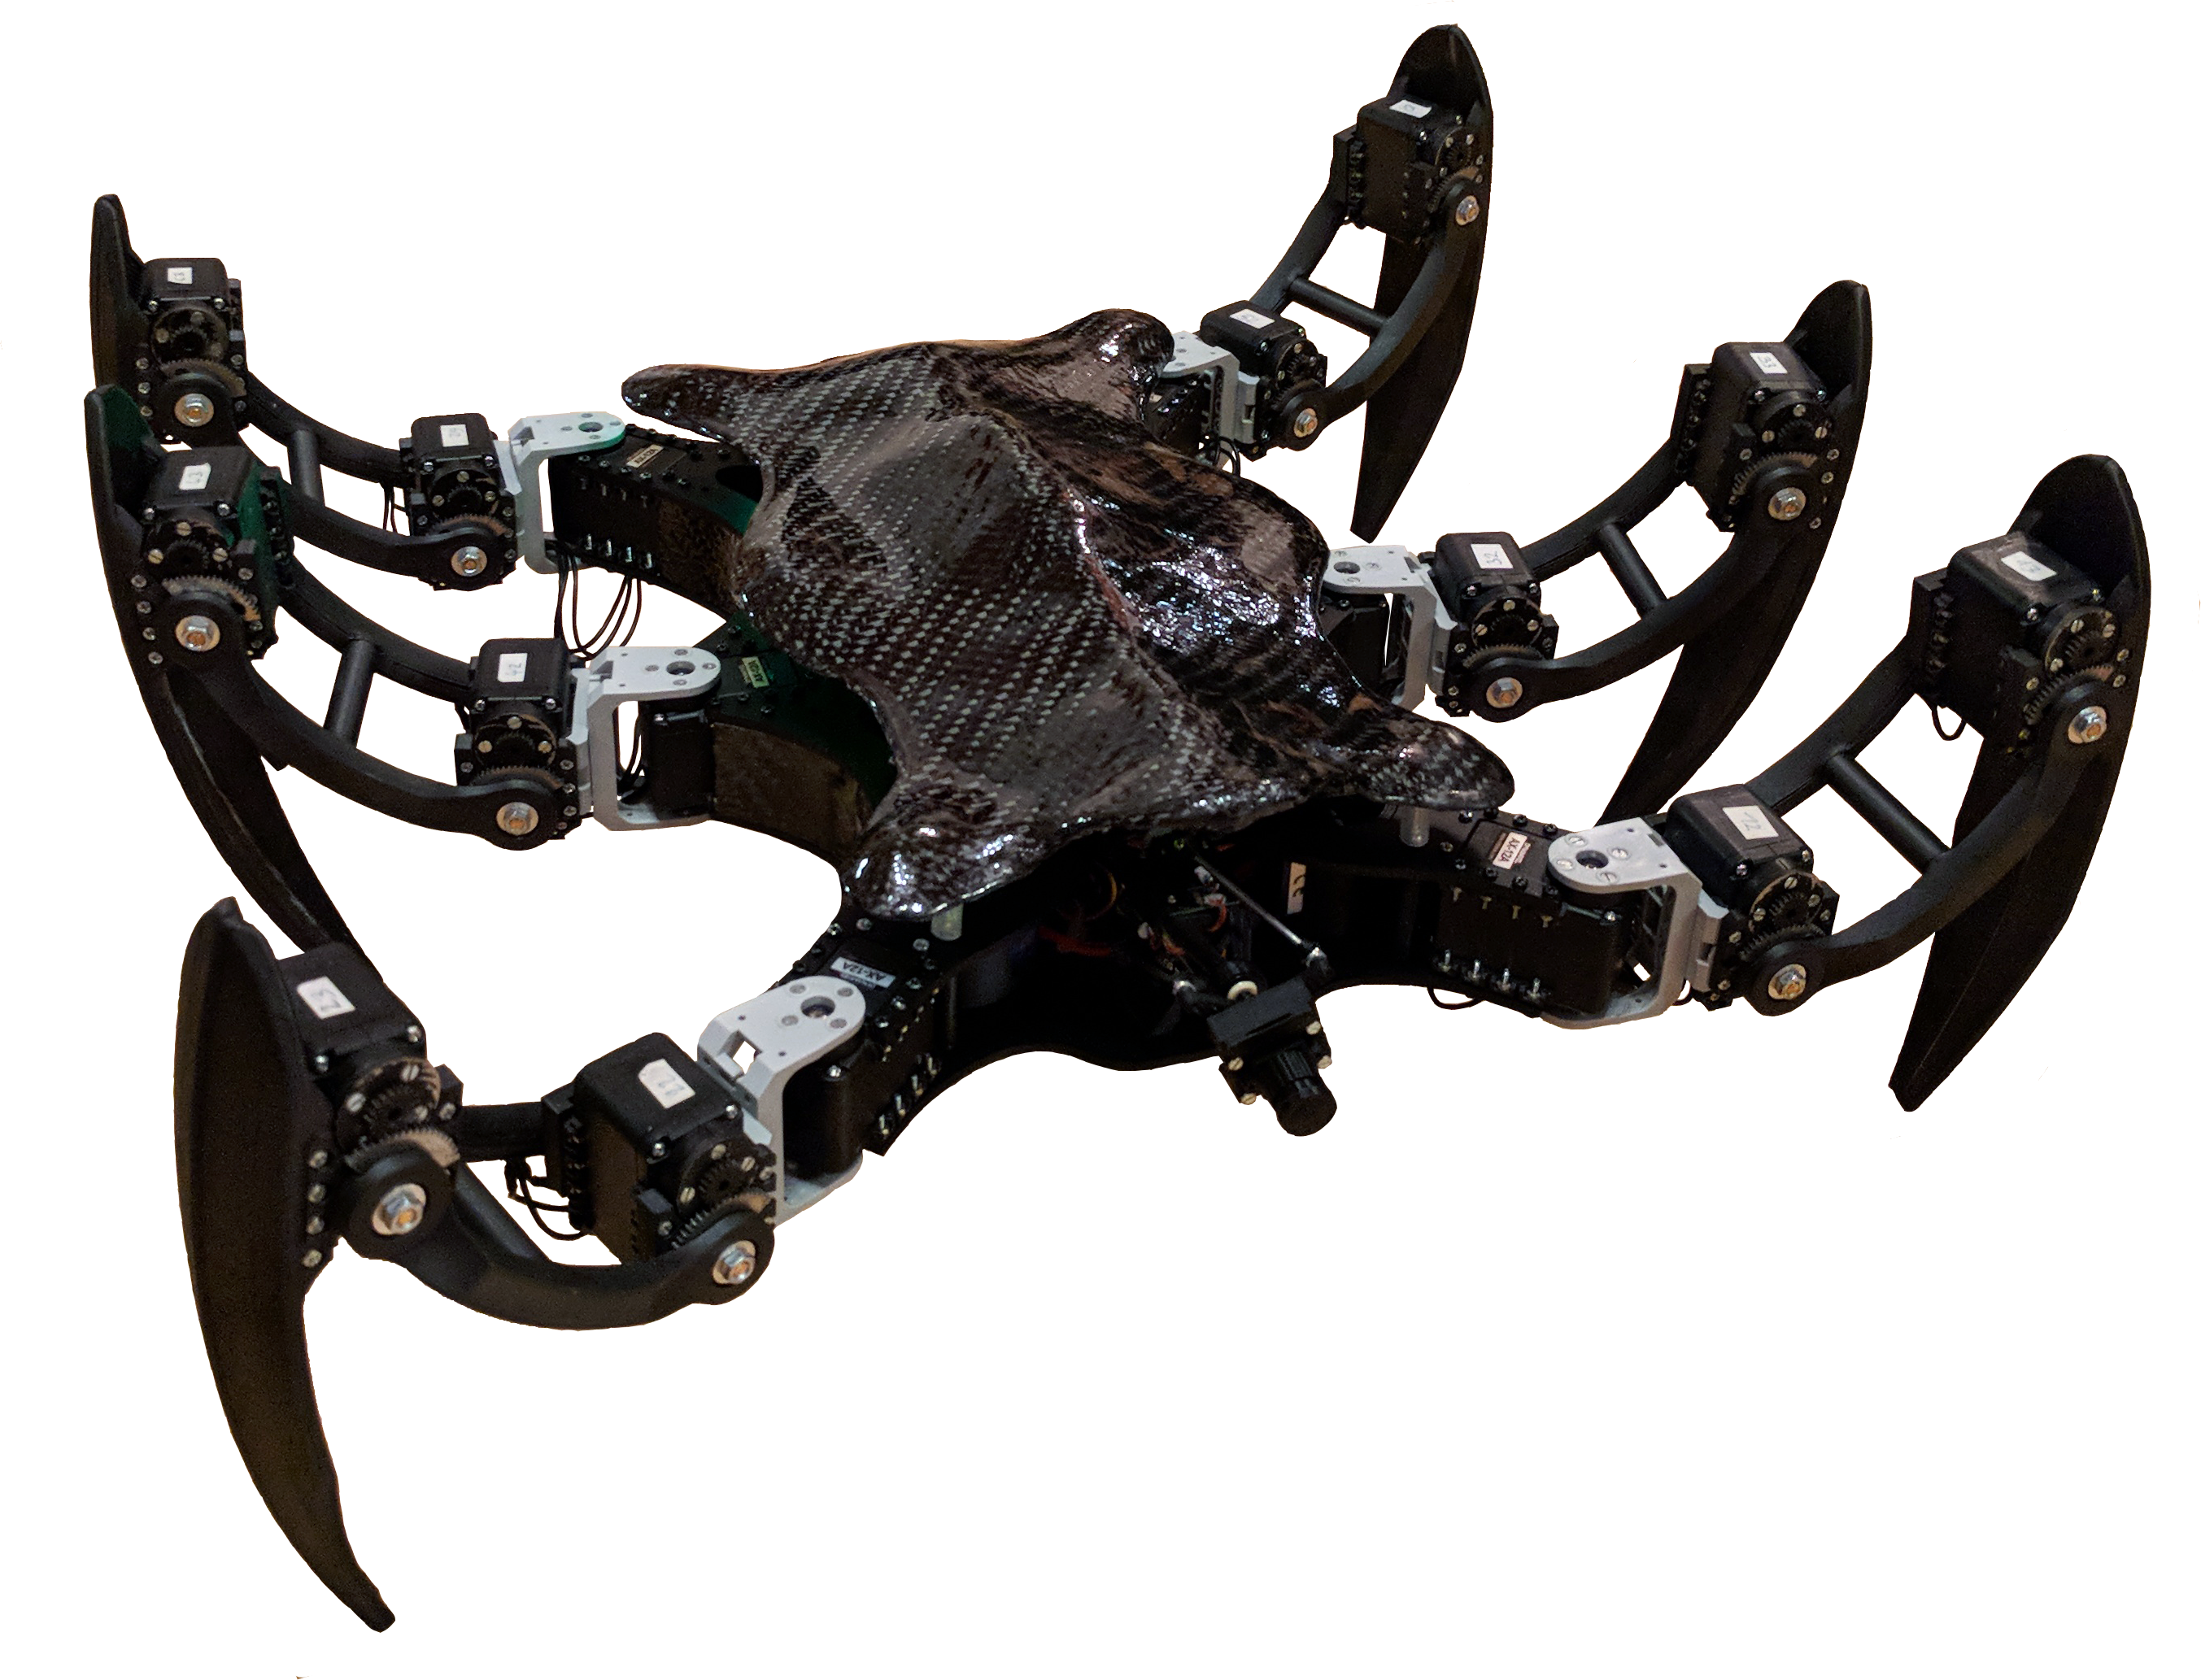
\includegraphics[width=7cm]{Hexapod.png}
\caption{Hexapod}
\label{fig:hexapod}
\end{center}
\end{figure}

Grafik neben Text:

\begin{wrapfigure}{R}{0.5\linewidth}
\includegraphics[scale=0.8]{GPE.png}
\caption{GP2Y0E03 \cite{GP2Y0E03}}
\label{fig:GPE}
\end{wrapfigure}

Lorem ipsum dolor sit amet, consectetur adipiscing elit, sed do eiusmod tempor incididunt ut labore et dolore magna aliqua. Ut enim ad minim veniam, quis nostrud exercitation ullamco laboris nisi ut aliquip ex ea commodo consequat. Duis aute irure dolor in reprehenderit in voluptate velit esse cillum dolore eu fugiat nulla pariatur. Excepteur sint occaecat cupidatat non proident, sunt in culpa qui officia deserunt mollit anim id est laborum. 
Lorem ipsum dolor sit amet, consectetur adipiscing elit, sed do eiusmod tempor incididunt ut labore et dolore magna aliqua. Ut enim ad minim veniam, quis nostrud exercitation ullamco laboris nisi ut aliquip ex ea commodo consequat. Duis aute irure dolor in reprehenderit in voluptate velit esse cillum dolore eu fugiat nulla pariatur. Excepteur sint occaecat cupidatat non proident, sunt in culpa qui officia deserunt mollit anim id est laborum. 


\section{Code Listings}
Code listings können mit verschiedenen packages erzeugt werden.

Code Listing:
\begin{lstlisting}[language=C++,caption=Example Code	]
  #include <stdio.h>
  
  int main (void) {
    printf("count: ");
    for (int i = 1; i <= 10; i++) {
     printf("%d ", i);
    }
    return 0;
  }
\end{lstlisting}


\bigskip
Alternatives Code Listing, floating, mit caption

\begin{listing}[H]
 \begin{minted}{c}
  #include <stdio.h>
  
  int main (void) {
    printf("count: ");
    for (int i = 1; i <= 10; i++) {
     printf("%d ", i);
    }
    return 0;
  }
  \end{minted}
  \caption{Example Code Caption}
\end{listing}

\bigskip 

Nicht Floating, ohne Caption:
\begin{minted}[label=``Example Code'']{c}
  #include <stdio.h>
  
  int main (void) {
    printf("count: ");
    for (int i = 1; i <= 10; i++) {
     printf("%d ", i);
    }
    return 0;
  }
\end{minted}



\section{Zitieren in Latex}
Latex nutzt Bibtex für die Verwaltung von Literaturquellen. In der Vorlage existiert bereits die Datei Literatur.bib mit zwei Einträgen. Ein Eintrag aus der Bibtex Datei kann mit mit \verb|\cite{key}| referenziert werden. Ein Beispiel: \cite{flegel}

Wird ein Eintrag aus Bibtex verwendet (zitiert), so scheint er im Quellenverzeichnis auf.
Zitieren von Websiten: \cite{htlwels}

Siehe \url{https://en.wikibooks.org/wiki/LaTeX/Bibliography_Management}

\chapter{Einleitung}
\label{sec:einleitung}


\section{Aufgabenstellung}
\label{sec:aufgabenstellung}




\chapter{Ideenfindung}
\label{sec:ideenfindung}


\section{Text}
\label{sec:text}



\chapter*{Anmerkung}

Diese Diplomarbeit wurde mittels LaTeX geschrieben, erstellt und formatiert.


Sämtliche LaTeX-Files sind auf dem beigelegten Speichermedium hinterlegt. Diese Dateien können für die Erstellung von weiteren Dokumentationen anderer Diplomarbeiten an der HTL-Wels verwendet werden.
\bigskip

\textbf{Distribution fuer Windows:}

MikTEX :    \url{http://miktex.org/2.9/setup}

\textbf{Editor:}

Texmaker : \url{https://www.xm1math.net/texmaker/download.html}




%### Abbildungsverzeichnis ###########################
\listoffigures

%### Tabellenverzeichnis #############################
%\listoftables

%### Abkuerzungsverzeichnis ##########################
\newpage
\chapter*{Abkürzungsverzeichnis}
\label{sec:Abkürzungsverzeichnis}

\begin{acronym}[MOSFET]
\acro{UART}{Universal Asynchronous Receiver Transmitter}
\acro{USB}{Universal Serial Bus}
\acro{PWM}{Pulsweitenmodulation}
\acro{bps}{Bits per Second}
\acro{I2C}{Inter-Integrated Circuit }
\acro{GPIO}{general purpose input/output}

\end{acronym}


%### Literaturverzeichnis ############################
\bibliographystyle{plain}
\bibliography{Literatur}

\pagestyle{empty}

%### Ende ############################################

\newpage
\begin{figure}
\begin{center}
\includegraphics[width=7cm]{HTLLogo.png}
\end{center}
\end{figure}

\vspace*{0cm}

\begin{center}
\Huge{\textbf{Diplomarbeit}}
\end{center}
\vspace*{-0.5cm}
\begin{figure}[h]
\begin{center}
\includegraphics[width=16cm]{ETverlauf.png}
\end{center}
\end{figure}


\begin{center}
\textbf{\Huge{Todo: Titel}}
\end{center}
  
  

  
  
  
  
  
  
    
\begin{figure}[b]
\begin{center}
\includegraphics[width=3cm]{HTLLogo2.png}
\end{center}
\end{figure}



\end{document}
